\fancypagestyle{periodic}{%
  \fancyhf{}%
  \fancyfoot[R]{\rotatebox{90}{\thepage}}%
  \renewcommand{\headrulewidth}{0pt}%
  \renewcommand{\footrulewidth}{0pt}%
}

\chapter{元素周期表　Periodic Table}\label{appendix:周期表}

    \section{元素周期表}\label{app:周期表-图表}

        \newgeometry{margin=0pt}
        \thispagestyle{periodic}
        \noindent
        \makebox[\textwidth][c]{\rotatebox{90}{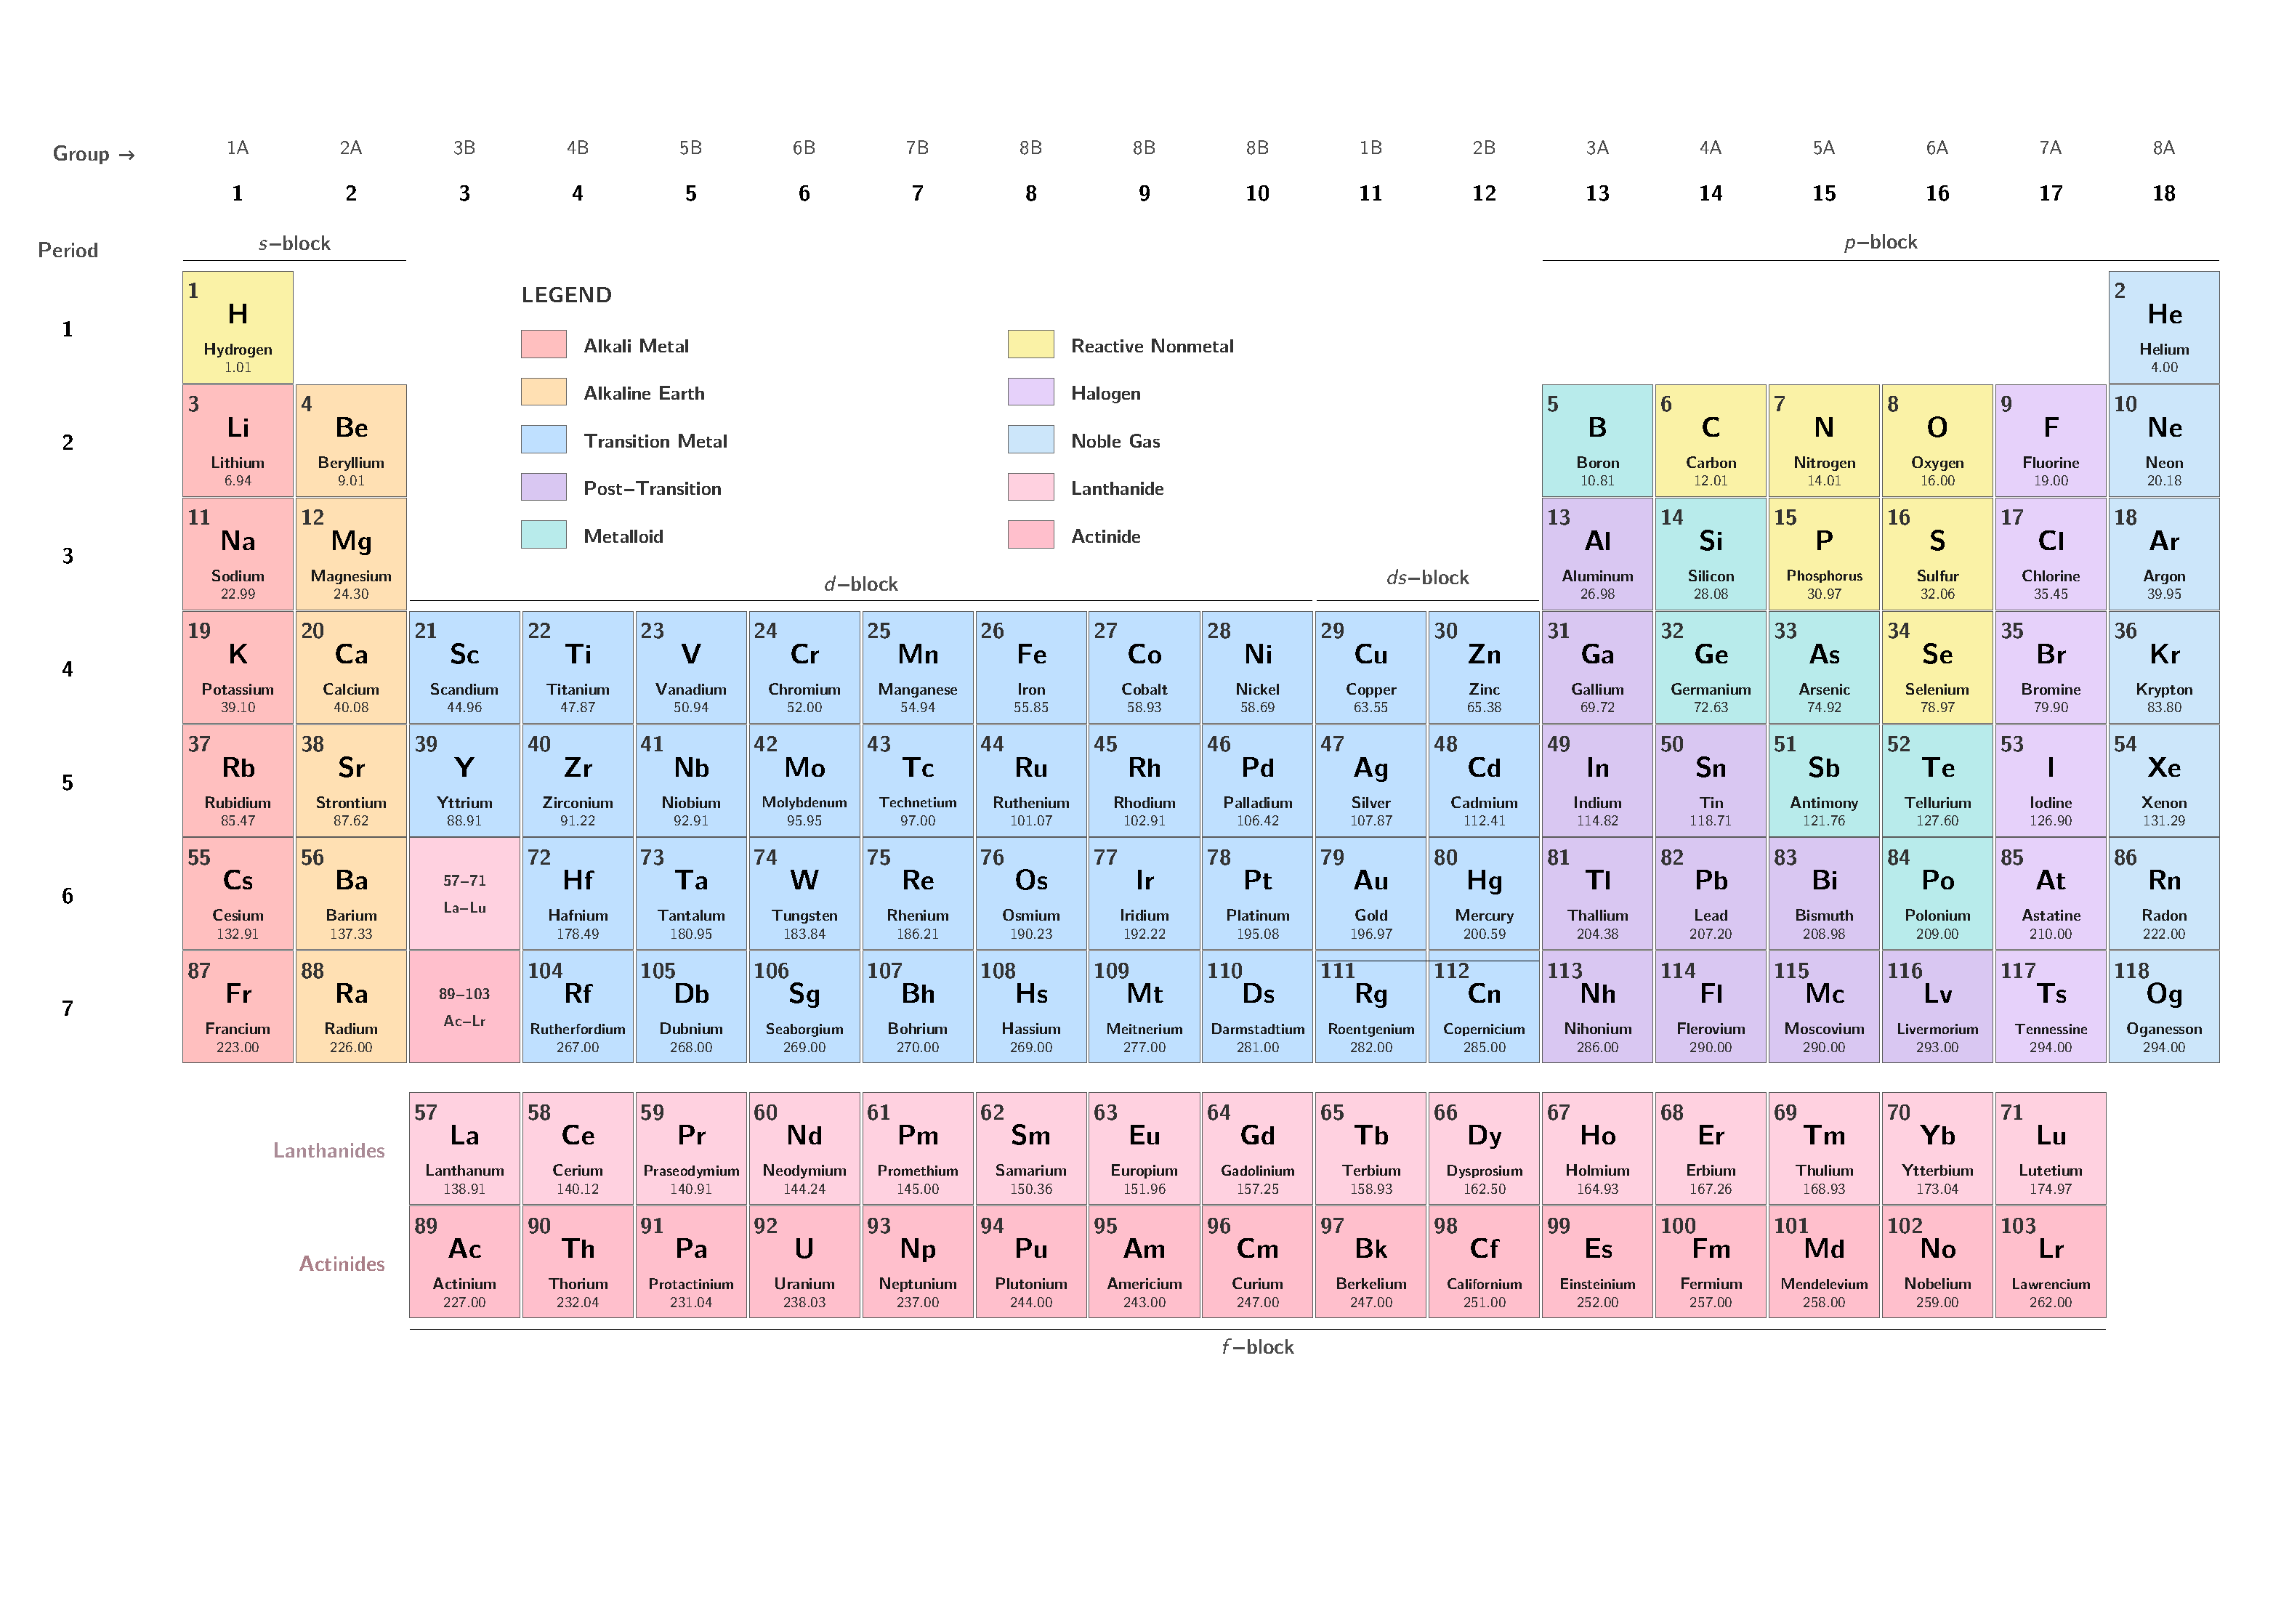
\includegraphics[width=\paperheight]{appendix/periodic-table.pdf}}}%
        \par
        \restoregeometry

    \section{元素周期律}\label{app:周期表-周期律}

        \begin{itemize}
            \item \textcolor{red}{周期律}：元素的性质随原子序数的递增而呈周期性变化。
            \item \textcolor{red}{原子半径}：同周期从左到右逐渐减小（核电荷数增大、电子层不变）；同主族从上到下逐渐增大（电子层增多）。
            \item \textcolor{red}{金属性/非金属性}：
            \begin{itemize}
                \item 同周期从左到右，金属性减弱、非金属性增强；
                \item 同主族从上到下，金属性增强、非金属性减弱。
            \end{itemize}
            \item \textcolor{red}{最高正化合价}：同周期从左到右，最高正价从 +1 递增到 +7（O、F 无正价）。
            \item \textcolor{red}{气态氢化物稳定性}：同周期从左到右增强（\cemh{CH4} \(<\) \cemh{NH3} \(<\) \cemh{H2O} \(<\) \cemh{HF}）；同主族从上到下减弱。
            \item \textcolor{red}{最高价氧化物对应水化物的酸碱性}：同周期从左到右酸性增强（碱性减弱）；同主族从上到下碱性增强（酸性减弱）。
            \item \textcolor{red}{电子层结构}：同周期电子层数相同；同主族最外层电子数相同（主族序数 \(=\) 最外层电子数）。
        \end{itemize}

    \section{背诵口诀}\label{app:周期表-口诀}

        \begin{itemize}
            \item \textcolor{blue}{主族序数}：主族序数 \(=\) 最外层电子数 \(=\) 最高正化合价。
            \item \textcolor{blue}{金属性判断}：失电子能力强则金属性强——与水或酸反应越剧烈、最高价氢氧化物碱性越强，金属性越强。
            \item \textcolor{blue}{非金属性判断}：得电子能力强则非金属性强——与 \cemh{H2} 化合越容易、气态氢化物越稳定、最高价含氧酸酸性越强，非金属性越强。
            \item \textcolor{blue}{半径规律}：先看电子层数（层多者半径大），同层再看核电荷数（核大者半径小），同核再看电子数（电子多者半径大）。
            \item \textcolor{blue}{对角线规则}：周期表中左上—右下对角线上的元素性质相似（如 \cemh{Li} 与 \cemh{Mg}、\cemh{Be} 与 \cemh{Al}）。
            \item \textcolor{blue}{同周期递变口诀}：金减非增，半径小，正价高，氢化物稳，酸性强
            \item \textcolor{blue}{同主族递变口诀}：金增非减，半径大，金属性强，氢化物不稳，碱性强
        \end{itemize}
